% ==================== 2.3 晶体的可视化 ====================
\subsection{晶体的可视化}

晶体结构是三维的，平面文字与二维投影图难以直观表达原子在空间中的排布、对称关系与配位
环境。晶体结构可视化软件（如 Diamond、VESTA、CrystalMaker 等）可将空间群、晶格常数与
原子坐标转化为可旋转、可缩放的三维模型，并支持晶面、配位多面体与粉末衍射谱的显示，
是学习晶体学的有力工具。下面以 Diamond 软件为例，介绍晶体结构的建模过程，并对八种常见
晶体结构逐一建模、图文讲解其结构特征\cite{diamond2023manual}。

\subsubsection{利用 Diamond 软件建立晶体结构模型}

本节以体心立方铁（空间群 $I\,m\,\bar3\,m$，$a=2.819$\,\AA）为例，说明从零开始建立
晶体结构模型的完整操作流程。

\textbf{（1）新建文档。}执行 File $\to$ New 命令，在弹出的 ``New Document'' 对话框中
选择 ``Create a document and type in or modify structure parameters''（创建一个文档并
输入或修改结构参数），如图~\ref{fig:dia-newdoc} 所示。

\begin{figure}[H]
  \centering
  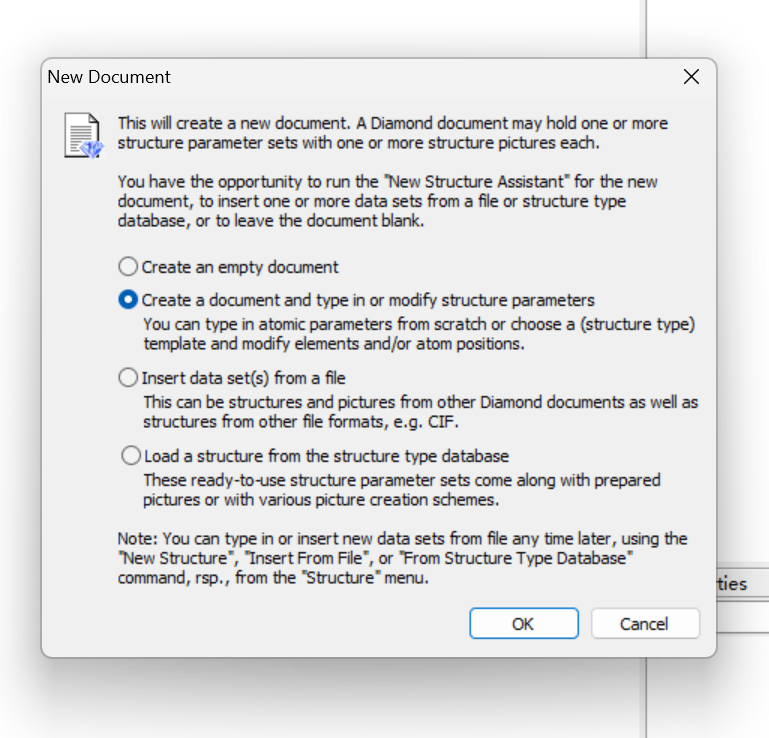
\includegraphics[width=0.52\textwidth]{assets/workflow/01-new-document.png}
  \caption{Diamond 软件的 New Document 对话框}
  \label{fig:dia-newdoc}
\end{figure}

\textbf{（2）选择晶体数据来源。}进入 ``New Structure'' 向导后，在 ``Source of structure
data'' 页选择 ``Type in new structure parameters''（输入新的结构参数），
如图~\ref{fig:dia-source} 所示。

\begin{figure}[H]
  \centering
  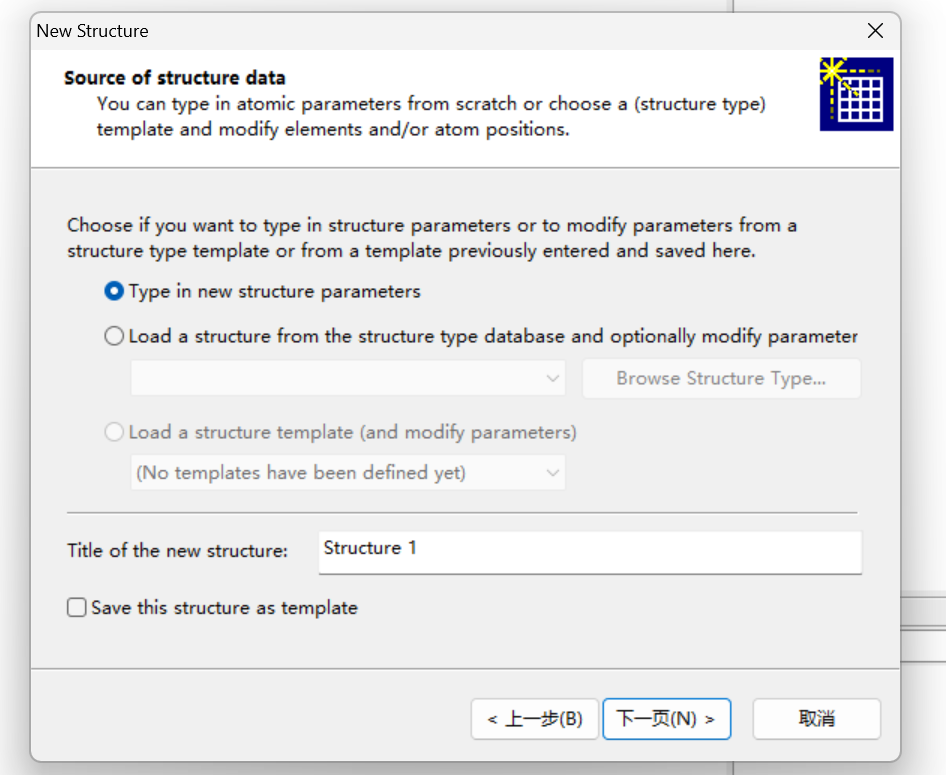
\includegraphics[width=0.52\textwidth]{assets/workflow/02-data-source.png}
  \caption{选择结构数据来源：直接输入新的结构参数}
  \label{fig:dia-source}
\end{figure}

\textbf{（3）设置空间群与晶格常数。}在 ``Cell parameters and space group'' 页通过
Browse 选择空间群（此处为 $I\,m\,\bar3\,m$ (229)），并输入晶格常数 $a$、$b$、$c$ 与
$\alpha$、$\beta$、$\gamma$（此处 $a=b=c=2.819$\,\AA，$\alpha=\beta=\gamma=90^\circ$），
如图~\ref{fig:dia-cell}(a) 所示。\textbf{注意事项}：空间群必须与晶系及晶格常数的关系
自洽，例如立方晶系要求 $a=b=c$ 且 $\alpha=\beta=\gamma=90^\circ$；若输入有误，可通过
Structure $\to$ Symmetry 修改空间群，再用 Build $\to$ Fill $\to$ Unit Cell 重建。

\textbf{（4）添加原子。}在 ``Atomic parameters'' 页输入元素种类与分数坐标 $x$、$y$、
$z$，点击 Add 将原子加入非对称单元，如图~\ref{fig:dia-cell}(b) 所示。通常只需输入
非对称单元中的不等价原子，Diamond 将依据空间群的对称操作自动生成晶胞内全部等价原子。

\begin{figure}[H]
  \centering
  \subcaptionbox{(a) 空间群与晶格常数设置\label{fig:dia-cell-a}}{%
    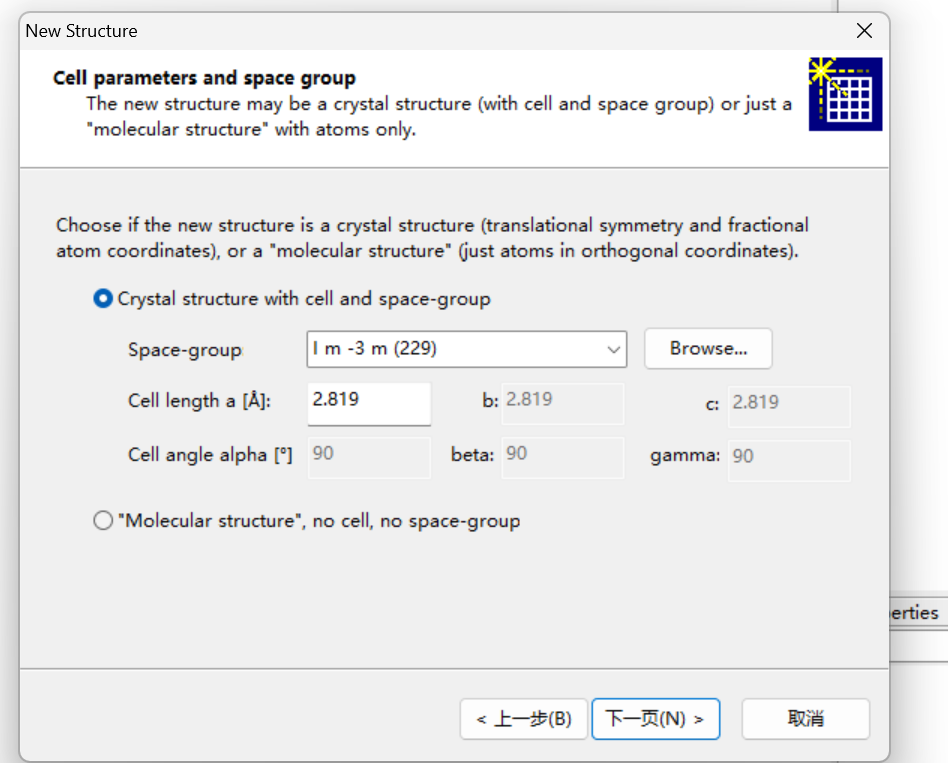
\includegraphics[width=0.44\textwidth]{assets/workflow/03-cell-parameters.png}}
  \hfill
  \subcaptionbox{(b) 原子参数（分数坐标）添加\label{fig:dia-cell-b}}{%
    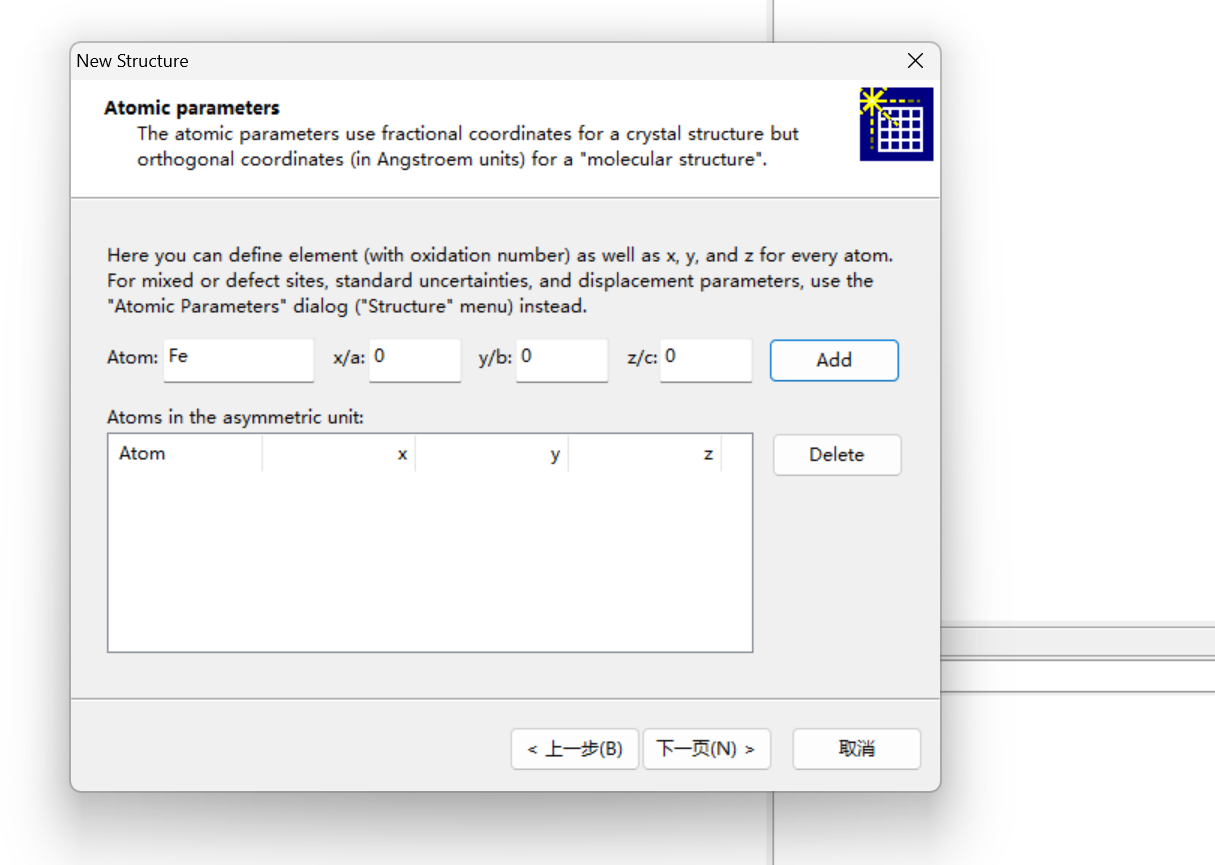
\includegraphics[width=0.46\textwidth]{assets/workflow/04-add-atoms.png}}
  \caption{Diamond 建模向导中的晶胞参数设置与原子添加}
  \label{fig:dia-cell}
\end{figure}

\textbf{（5）填充晶胞与扩展显示。}执行 Build $\to$ Fill $\to$ Unit Cell 生成一个晶胞的
结构模型；执行 Build $\to$ Fill $\to$ Box（或 Range）可显示多个相邻晶胞，以便观察结构
的周期延伸；若需恢复单胞显示，删除全部原子后用 Unit Cell 重建即可。

\textbf{（6）视图与外观设置。}按住鼠标拖动可实时旋转、缩放模型，选择合适的观察方向；
右键原子执行 Edit $\to$ Atom Design 可设置原子颜色与显示半径；选中原子后右键执行
Add $\to$ Atom Labels，可将标签类型设为 Atom Identifier、格式设为 ATOM \#，给原子编号，
便于追踪对称操作前后原子的对应关系。

\textbf{（7）建立晶面。}执行 Objects $\to$ Planes $\to$ Create Lattice Plane，输入
Miller 指数 $(h\,k\,l)$ 与位置（以 $d$ 间距的倍数表示），即可在模型中添加晶面，
如图~\ref{fig:dia-plane} 所示（图中为 BCC 铁的 (111) 晶面，$d=1.6276$\,\AA）。在右侧
Tables of Planes 面板中右键某晶面可进入 Shift Plane Mode，沿晶面法线方向拖动晶面；
执行 Build $\to$ Fill $\to$ Slab 则可显示晶面及其上下指定范围内的原子，便于观察密排面。

\begin{figure}[H]
  \centering
  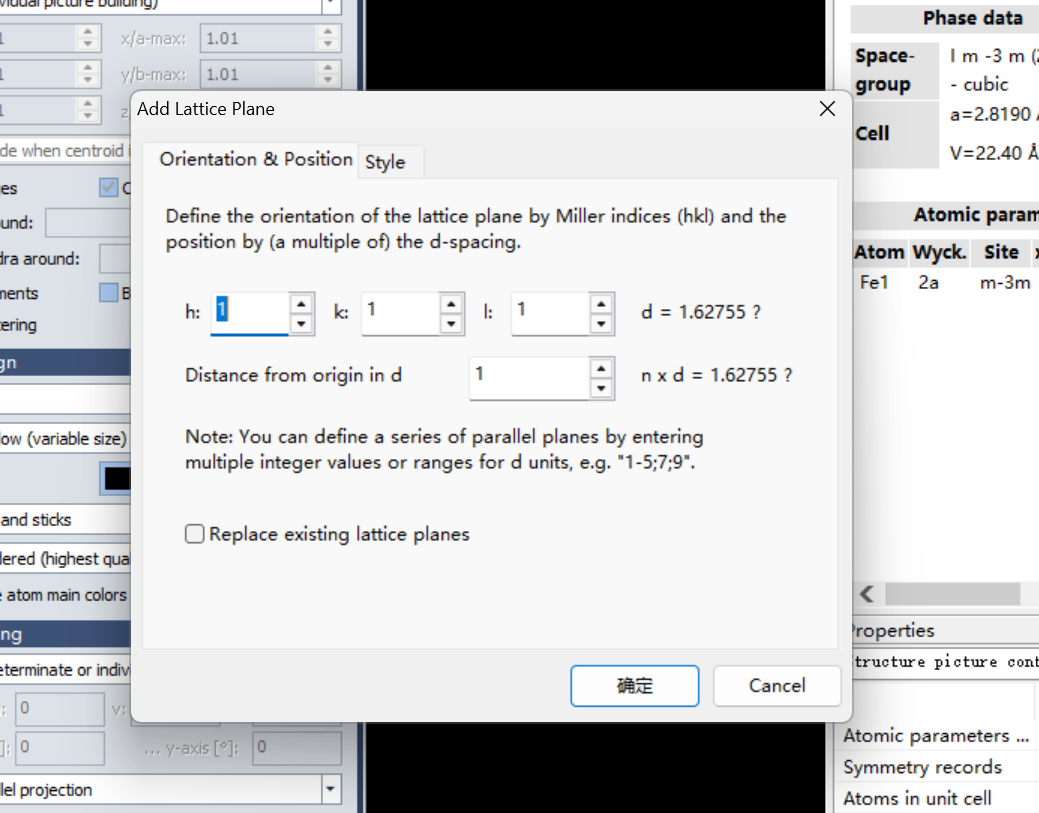
\includegraphics[width=0.52\textwidth]{assets/workflow/08-add-lattice-plane.png}
  \caption{Add Lattice Plane 对话框：输入 Miller 指数与晶面位置}
  \label{fig:dia-plane}
\end{figure}

\textbf{（8）添加配位多面体。}执行 Build $\to$ Polyhedra $\to$ Add Coordination
Polyhedra，在对话框中选择中心原子与配位原子并设置键长范围，即可显示配位多面体，
如图~\ref{fig:dia-poly} 所示。若只想观察特定原子的配位环境，可先选中该原子作为中心再
调用此功能。通过观察配位多面体之间共角、共棱、共面的连接方式，可以理解配位体如何
堆积、键合进而形成晶体（三种连接方式的稳定性依次降低）。

\begin{figure}[H]
  \centering
  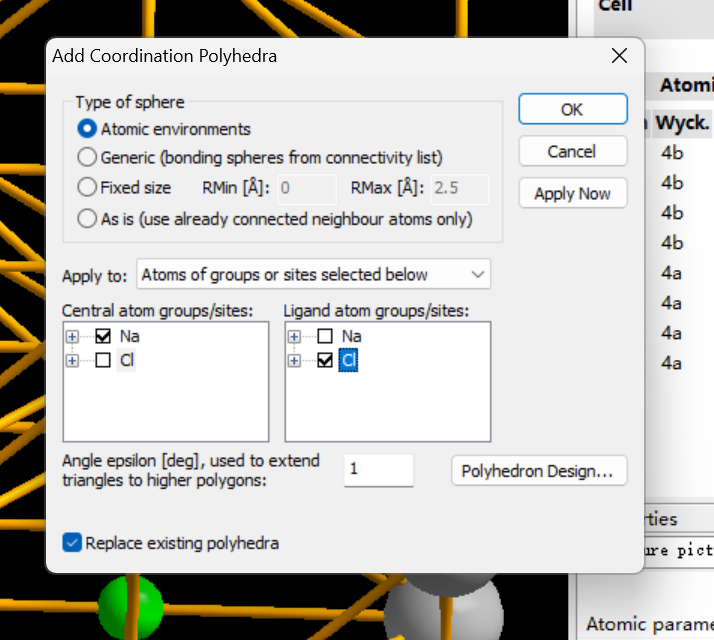
\includegraphics[width=0.46\textwidth]{assets/workflow/09-add-coordination-polyhedra.png}
  \caption{Add Coordination Polyhedra 对话框：选择中心原子与配位原子}
  \label{fig:dia-poly}
\end{figure}

\textbf{（9）模拟 X 射线粉末衍射图。}执行 View $\to$ Powder Pattern
（图~\ref{fig:dia-xrd}(a)），在衍射设置中选择 X 射线模式、波长与 $2\theta$ 范围等参数
（图~\ref{fig:dia-xrd}(b)(c)），即可得到该晶体结构的理论粉末衍射谱，用于与实际 XRD
图谱对比。

\begin{figure}[H]
  \centering
  \subcaptionbox{(a) View 菜单中的 Powder Pattern 命令}{%
    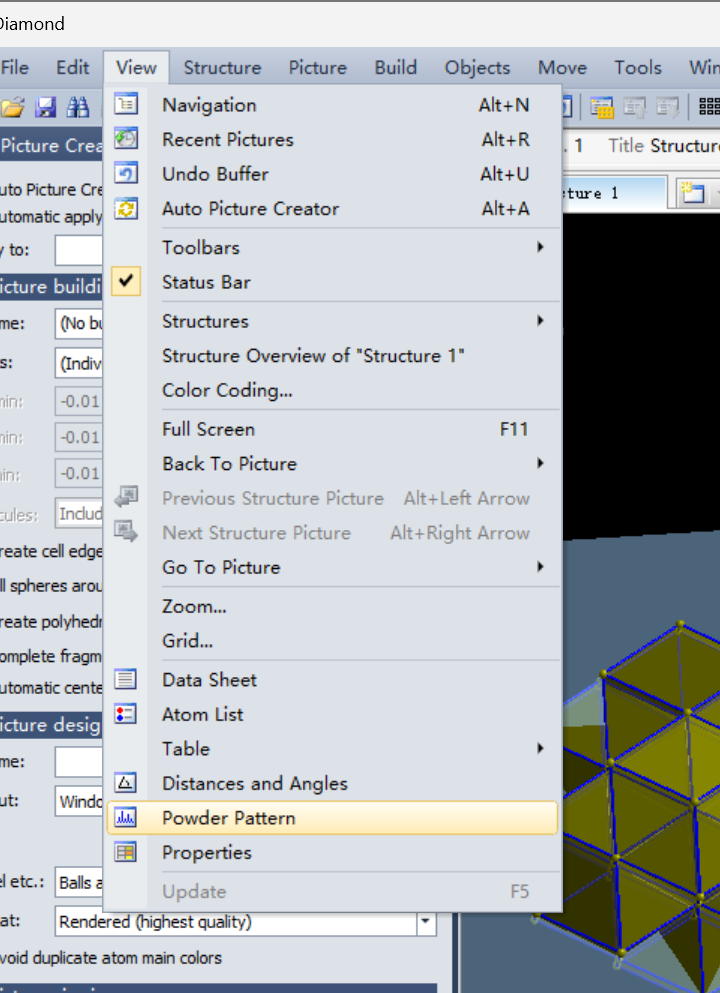
\includegraphics[width=0.30\textwidth]{assets/workflow/05-view-powder-pattern.png}}
  \hfill
  \subcaptionbox{(b) 选择 XRD 衍射模式}{%
    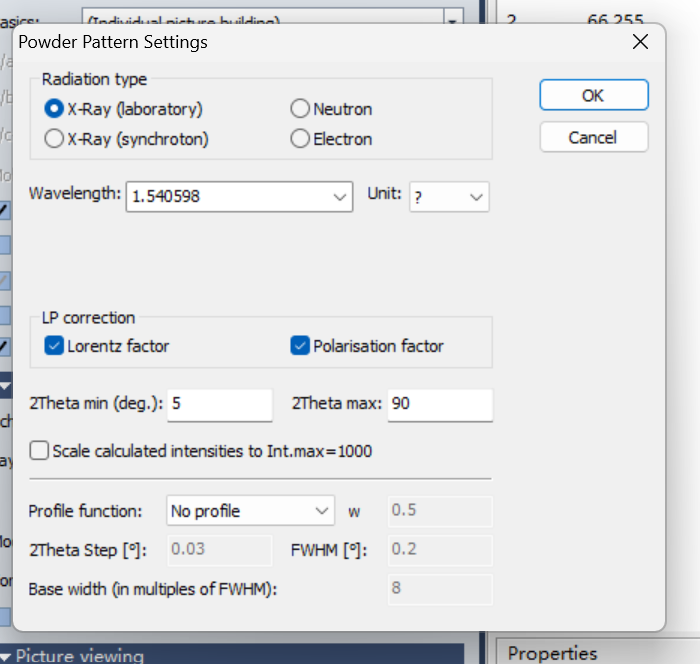
\includegraphics[width=0.30\textwidth]{assets/workflow/06-xrd-mode.png}}
  \hfill
  \subcaptionbox{(c) XRD 模拟参数设置}{%
    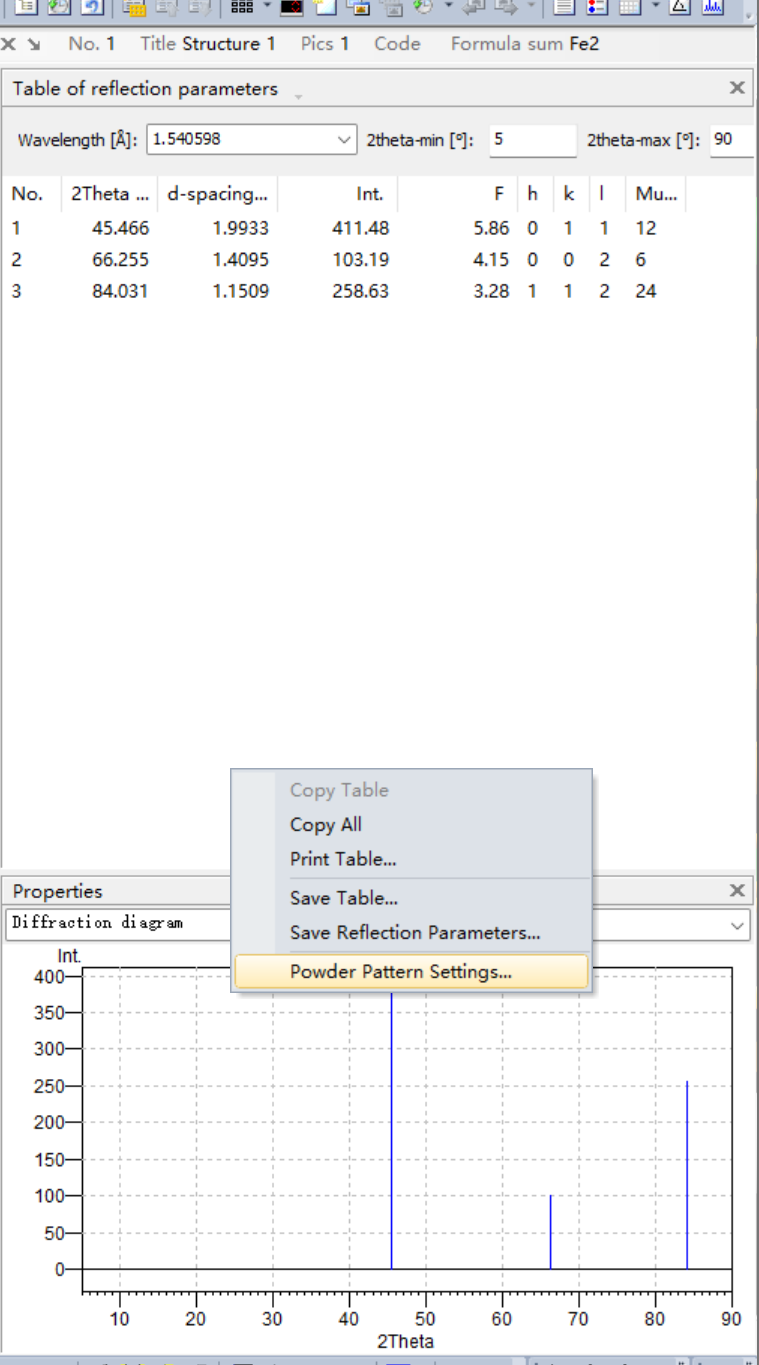
\includegraphics[width=0.30\textwidth]{assets/workflow/07-xrd-settings.png}}
  \caption{Diamond 中粉末衍射图的模拟}
  \label{fig:dia-xrd}
\end{figure}

\textbf{（10）测量工具。}利用 Tools 菜单中的距离与角度测量功能，可测定键长、键角与
晶面间距，用于定量验证结构特征。

归纳起来，Diamond 建模与观察的要点包括：空间群、晶系与晶格常数必须自洽；原子坐标采用
分数坐标，只需输入非等效原子；统计晶胞内原子数时，顶点原子计 $1/8$、棱上原子计 $1/4$、
面上原子计 $1/2$、内部原子计 $1$；在钢球模型下，先找密排方向（密排线），由原子相切
条件求出原子半径，即可计算原子堆积因子（体积占有率）；配位多面体的连接方式（共角、
共棱、共面）反映了配位体堆积的稳定性。

\subsubsection{常见晶体结构的特征}

下面利用上述建模方法，对八种常见晶体结构逐一建立模型并讲解其结构特征。每种结构均给出
建模参数（空间群、晶格常数、非对称单元原子坐标与化学式单元数 $Z$），并结合结构模型图、
理论粉末衍射图、密堆积晶面图与配位多面体图进行分析；文中所有截图均由 Diamond 软件生成。
